\documentclass[border=3pt]{standalone}
% Preâmbulo compartilhado pelos diagramas TikZ da aula 4 de Navegação (Representação de Mapas)
\usepackage[T1]{fontenc}
\usepackage[utf8]{inputenc}
\usepackage{lmodern}
\usepackage{amsmath}
\usepackage{xcolor}
\usepackage{tikz}
\usetikzlibrary{arrows.meta,angles,quotes,decorations.pathmorphing,decorations.pathreplacing,calc,
                positioning,shapes.geometric,shapes.misc,backgrounds,fit,
                math}

% Paleta (mesma dos SVGs originais)
\definecolor{dblue}{HTML}{2A5B8C}
\definecolor{dorange}{HTML}{B3541E}
\definecolor{dgreen}{HTML}{4A7C59}
\definecolor{dred}{HTML}{9C4B4B}
\definecolor{dcream}{HTML}{F4F1EA}
\definecolor{dshade}{HTML}{DDD7C9}

% Função gaussiana (não normalizada por padrão de escala visual)
\pgfmathdeclarefunction{gauss}{3}{%
  \pgfmathparse{1/(#3*sqrt(2*pi))*exp(-((#1-#2)^2)/(2*#3^2))}%
}

% Estilos comuns (prefixo d... para não colidir com chaves internas do pgf)
\tikzset{
  >={Stealth[length=2mm]},
  dguide/.style={gray!55, dashed, line width=0.4pt},
  daxis/.style={gray!60, line width=0.7pt, ->},
  dbody/.style={fill=black!3, draw=black!80, line width=1pt},
  dacc/.style={draw=dblue, line width=1pt},
  dlbl/.style={black!55, font=\small},
  dsub/.style={black!45, font=\footnotesize},
  dstate/.style={circle, draw=black!80, fill=dcream, line width=1pt,
                 minimum size=17mm, font=\large, inner sep=1pt},
  dobs/.style={circle, draw=black!80, fill=dshade, line width=1pt,
               minimum size=14mm, font=\large, inner sep=1pt},
  dbox/.style={rounded corners=2pt, draw=black!80, fill=dcream, line width=1pt,
               align=center, inner sep=6pt},
  dop/.style={circle, draw=black!80, fill=white, line width=1pt,
              minimum size=6mm, inner sep=0pt, font=\small},
  dtrans/.style={->, dblue, line width=1pt},
  dmeas/.style={->, dorange, line width=1pt},
  dcurve/.style={line width=1pt, dblue},
  dcurveb/.style={line width=1.4pt, dorange},
}

\begin{document}
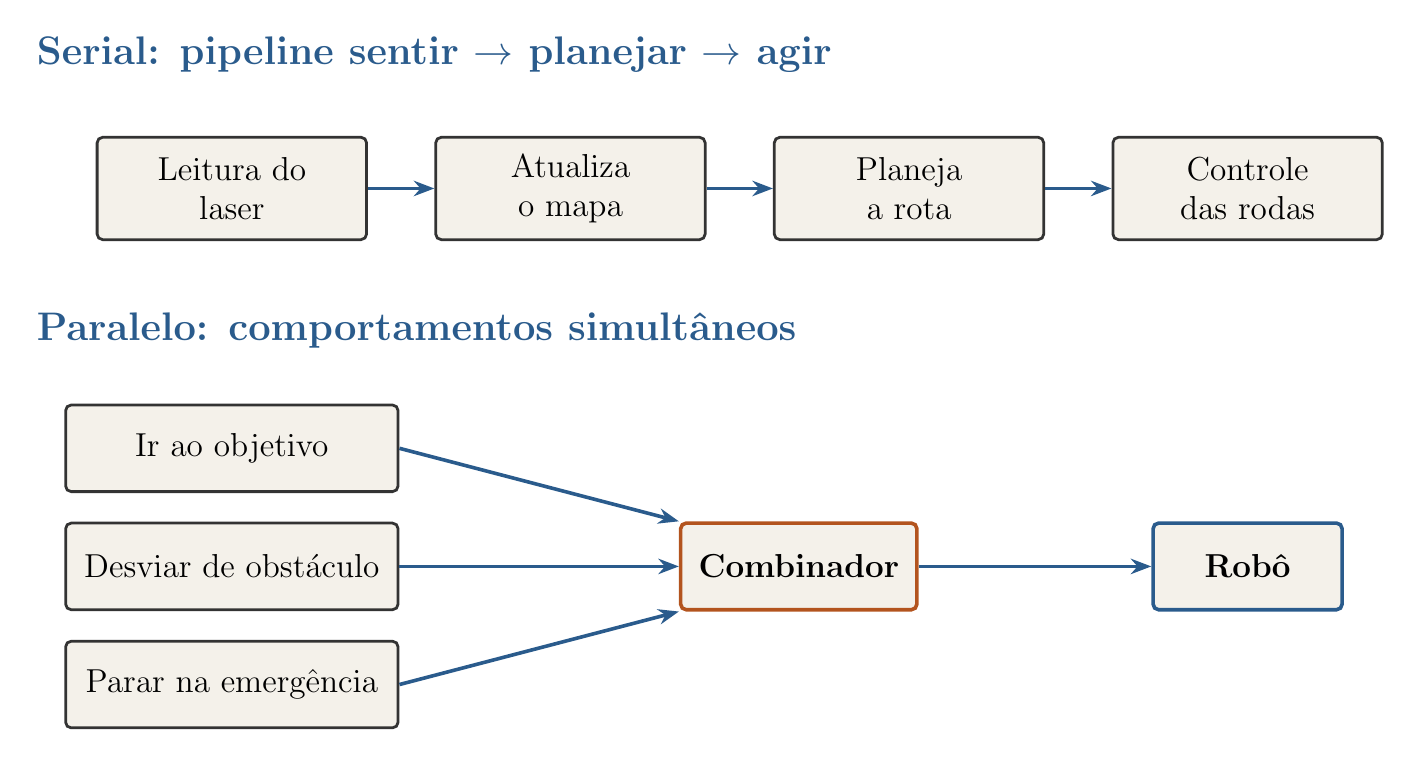
\begin{tikzpicture}[x=1cm,y=1cm]

  \tikzset{mod/.style={dbox, minimum width=3.8cm, text width=3.8cm, minimum height=1.1cm, font=\large, align=center},
           rob/.style={dbox, minimum width=2.4cm, minimum height=1.1cm, font=\large\bfseries, draw=dblue, line width=1.3pt},
           comb/.style={dbox, minimum width=3.0cm, minimum height=1.1cm, font=\large\bfseries, draw=dorange, line width=1.3pt}}

  % ---------- Serial: sentir -> mapear -> planejar -> controlar ----------
  \node[font=\bfseries\Large, dblue, anchor=west] at (-0.8,5.4) {Serial: pipeline sentir $\to$ planejar $\to$ agir};
  \node[mod, minimum width=3.0cm, text width=3.0cm, minimum height=1.3cm] (a1) at (1.8,3.7) {Leitura do\\laser};
  \node[mod, minimum width=3.0cm, text width=3.0cm, minimum height=1.3cm] (a2) at (6.1,3.7) {Atualiza\\o mapa};
  \node[mod, minimum width=3.0cm, text width=3.0cm, minimum height=1.3cm] (a3) at (10.4,3.7) {Planeja\\a rota};
  \node[mod, minimum width=3.0cm, text width=3.0cm, minimum height=1.3cm] (a4) at (14.7,3.7) {Controle\\das rodas};
  \draw[dtrans, line width=1.3pt, -{Stealth[length=2.6mm]}] (a1) -- (a2);
  \draw[dtrans, line width=1.3pt, -{Stealth[length=2.6mm]}] (a2) -- (a3);
  \draw[dtrans, line width=1.3pt, -{Stealth[length=2.6mm]}] (a3) -- (a4);

  % ---------- Paralelo: comportamentos ----------
  \begin{scope}[shift={(0,1.0)}]
  \node[font=\bfseries\Large, dblue, anchor=west] at (-0.8,0.9) {Paralelo: comportamentos simultâneos};
  \node[mod] (b1) at (1.8,-0.6) {Ir ao objetivo};
  \node[mod] (b2) at (1.8,-2.1) {Desviar de obstáculo};
  \node[mod] (b3) at (1.8,-3.6) {Parar na emergência};
  \node[comb] (n) at (9.0,-2.1) {Combinador};
  \node[rob] (r) at (14.7,-2.1) {Robô};
  \draw[dtrans, line width=1.3pt, -{Stealth[length=2.6mm]}] (b1.east) -- (n.north west);
  \draw[dtrans, line width=1.3pt, -{Stealth[length=2.6mm]}] (b2.east) -- (n.west);
  \draw[dtrans, line width=1.3pt, -{Stealth[length=2.6mm]}] (b3.east) -- (n.south west);
  \draw[dtrans, line width=1.3pt, -{Stealth[length=2.6mm]}] (n) -- (r);
  \end{scope}

\end{tikzpicture}
\end{document}
